Una vez identificados los interesados tanto directos como indirectos y los requisitos del sistema se procederá a realizar una descomposición en subsistemas.  Cada subsistema tendrá una funcionalidad única y acotada.

A continuación se detalla cada uno de los subsistemas identificados:

\begin{description}
\item[Subsistema de búsqueda]  El subsistema de búsqueda es el encargado de gestionar todas las búsquedas que realicen los usuarios y retornar los resultados convenientes.  Además también se encargará de indexar periódicamente (o puntualmente si un administrador lo desea) los contenidos del portal.
\item[Subsistema de gestión de usuarios]  Éste subsistema será el encargado de gestionar todas las operaciones que se realizan relacionadas con los datos de un usuario.  Algunas de las tareas gestionadas por este subsistema son los registros, los inicios de sesión o la asignación de diferentes roles de usuario.
\item[Subsistema de gestión de debates]  Éste subsistema se encargará de gestionar todas las operaciones relacionadas con los debates, desde la creación y modificación de nuevos debates hasta la apertura o cierre de los debates ya existentes y la gestión de los comentarios de los usuarios.
\item[Subsistema de gestión de eventos]  Éste subsistema se encargará de gestionar todas las operaciones que guarden relación con los eventos.  Las tareas típicas de éste subsistema serán la creación y la edición de eventos.
\item[Subsistema de gestión de noticias]  Éste subsistema se encargará de gestionar las operaciones relacionadas con las noticias, principalmente la creación y edición de noticias.
\item[Subsistema de gestión del blog]  Éste subsistema se encargará de gestionar las tareas relacionadas con las entradas del blog.  Algunas funciones de éste subsistema serán la creación y edición de entradas en el blog y la moderación de los comentarios de usuarios.
\item[Subsistema de gestión de organizaciones]  Éste subsistema se encargará de gestionar las tareas relacionadas con las organizaciones, principalmente la creación, edición y eliminación de noticias.
\item[Subsistema de gestión de datos]  Éste subsistema será el encargado de gestionar los datos de la parte de datos del portal.  Las funciones más representativas de éste subsistema son la inserción de nuevos catálogos de datos y la provisión de información con la que crear las visualizaciones.
\item[Subsistema de gestión de comentarios]  Éste subsistema será el encargado de gestionar los comentarios de los usuarios.  Las funciones más representativas de este subsistema son la creación, la modificación y la eliminación de comentarios.
\end{description}

Es necesario tener en cuenta que el sistema final que será el nuevo Land Portal contará con más subsistemas que no son objeto de éste proyecto y, por tanto, no figuran en éste análisis.


\subsection{Descripción de las interfaces entre subsistemas}
Tras haber realizado la identificación de los subsistemas  se describirá de qué forma se relacionarán dichos subsistemas.

Todos los subsistemas mencionados anteriormente se encontrarán en el mismo servidor web, aunque formarán parte de diferentes aplicaciones y componentes.  Concretamente:
\begin{itemize}
\item Los subsistemas de gestión de usuarios, debates, eventos, noticias, entradas del blog y comentarios formarán parte del gestor de contenidos o CMS.  A lo largo de ésta documentación el conjunto de todos estos subsistemas recibirá también el nombre de ``zona social''.
\item El subsistema de búsqueda formará parte del buscador que, como se ha explicado en la sección \nameref{chapter02:alternativas_seleccionadas} perteneciente al capítulo \ref{chapter02:alternativas_seleccionadas} sera Apache Solr.
\item El subsistema de gestión de datos estará dividido entre una aplicación encargada de la inserción de datos provenientes de fuentes externas y un framework que dará soporte a las visualizaciones de datos.  Por su funcionalidad, éste subsistema también recibirá el nombre de ``zona de datos'' en ésta documentación.
\end{itemize}

Los subsistemas que forman parte del gestor de contenidos (gestión de usuarios, debates, eventos, noticias, entradas del blog y comentarios) se comunicarán con el subsistema de búsqueda a través del API HTTP ofrecido por el buscador. \newline
Por otra parte el gestor de contenidos y el subsistema de gestión de datos se comunicarán a través de una base de datos compartida, será el gestor de contenidos quien extraiga los datos necesarios de la base de datos en la que el subsistema de gestión de datos almacena la información.

En la imagen \ref{fig:diagrama_subsistemas} se puede ver un esquema que representa la situación de dichos componentes y subsistemas.

\begin{figure}[h]
\centering
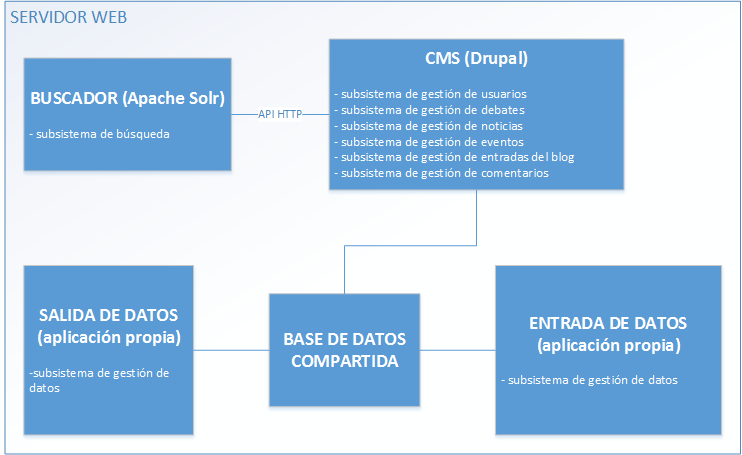
\includegraphics[width=\textwidth]{subsistemas/diagrama_subsistemas}
\caption{Diagrama de subsistemas}
\label{fig:diagrama_subsistemas}
\end{figure}